\defn. \note{Algebraic Extension} Let \(E\) be an extension field of \(F\). \(E\) is an \textbf{algebraic extension} of \(F\) if all elements in \(E\) are algebraic over \(F\).

\begin{center}
    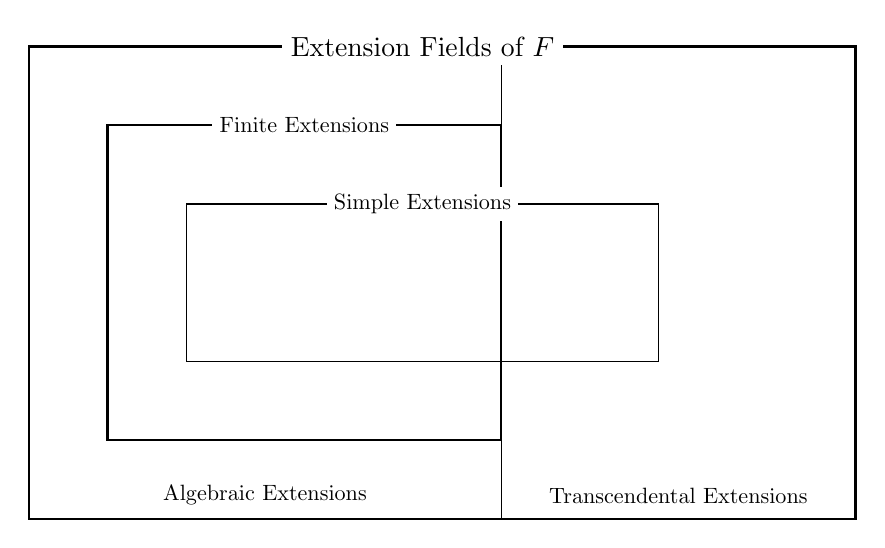
\begin{tikzpicture}
        \draw[thick] (0, 0) rectangle (10.5, 6);
        \draw (6, 0) -- (6, 6);
        \draw (2, 2) rectangle (8, 4);
        \draw[thick] (1, 1) rectangle (6, 5);
        \node[fill=white] at (5, 6) {Extension Fields of \(F\)};
        \node[fill=white, scale=0.8] at (3, 0.3) {Algebraic Extensions};
        \node[fill=white, scale=0.8] at (8.25, 0.3) {Transcendental Extensions};
        \node[fill=white, scale=0.8] at (3.5, 5) {Finite Extensions};
        \node[fill=white, scale=0.8] at (5, 4) {Simple Extensions};
    \end{tikzpicture}
\end{center}

\thm. Every finite extension is an algebraic extension.

\pf Let \(E\) be a finite extension of degree \(n\) over \(F\). Take \(\alpha \in E\). Then \(\{1, \alpha, \dots, \alpha^{n-1}, \alpha^n\}\) is linearly dependent over \(F\).\footnote{Recall from linear algebra: if \(\dim_F E = n\), then any subset of \(E\) with more than \(n\) elements is linearly dependent over \(F\).} Then we can choose \(b_0, \dots, b_n \in F\) such that
\begin{center}
    \(b_0 + b_1 \alpha + \cdots + b_n\alpha^n = 0\) and \(b_i \neq 0\) for some \(i\).
\end{center}
Equivalently, if we set \(f(x) = b_0 + b_1 x + \cdots + b_n x^n \in F[x]\), then \(f(x) \neq 0\) and \(f(\alpha) = 0\). Thus any element \(\alpha \in E\) is algebraic. \qed

\cor. If \(\alpha \in E\) is algebraic over \(F\) then \(F(\alpha)\) is an algebraic extension.

\thm. Let \(E\) be a finite extension over \(F\), and \(K\) be a finite extension over \(E\). Then
\[
    [K: F] = [K : E] [E : F].
\]

\pf Set \(m = [K : E]\), \(n = [E : F]\). Let \(\{\alpha_1, \dots, \alpha_n\}\) be an \(F\)-basis of \(E\) and \(\{\beta_1, \dots, \beta_m\}\) be an \(E\)-basis of \(K\). Now we show that
\[
    \mf{B} = \{\alpha_i \beta_j : 1 \leq i \leq n,\, 1 \leq j \leq m\}
\]
is an \(F\)-basis of \(K\).
\begin{itemize}
    \item (\(\mf{B}\) spans \(K\) over \(F\)) Check by yourself.
    \item (\(\mf{B}\) is linearly independent) Suppose for \(c_{ij} \in F\), we have \(\sum_{i, j} c_{ij}\alpha_i\beta_j = 0\). Then we can write
    \[
        \sum_{i, j} c_{ij}\alpha_i\beta_j = \sum_{j}\paren{\sum_{i} c_{ij}\alpha_i}\beta_j = 0.
    \]
    Since \(\beta_j\) are linearly independent, \(\sum_i c_{ij} \alpha_i = 0\) for all \(j\). In the same way, linear independence of \(\alpha_i\) gives \(c_{ij} = 0\) for all \(i, j\). \qed
\end{itemize}

Let \(\tilde{F}\) be an extension field of \(F\) and let \(\alpha \in \tilde{F}\) be algebraic. Then \(E = F(\alpha)\) is a simple, finite extension. Take another element \(\beta \in E\), that is algebraic in an extension field \(\tilde{E}\). Then to describe \(E(\beta)\), we can split the field into two simple extensions,
\[
    [E(\beta) : F] = \overbrace{[E(\beta) : E]}^{\text{simple}} \overbrace{[F(\alpha) : F]}^{\text{simple}}.
\]
and inspect each simple extension.

\cor. Let \(F_{i+1}\) be a finite extension field over \(F_i\) for \(i = 1, \dots, r - 1\). Then \(F_r\) is a finite extension of \(F_1\) and
\[
    [F_r : F_1] = [F_r : F_{r - 1}] [F_{r - 1} : F_{r - 2}] \cdots [F_2 : F_1].
\]

\cor. Let \(\alpha \in E\) be algebraic over \(F\). If \(\beta \in F(\alpha)\), then \(\deg(\beta, F) \mid \deg(\alpha, F)\).

\pf \(F \subset F(\alpha)\), \(\beta \in F(\alpha)\), so \(F(\beta) \subset F(\alpha)\) since \(F(\beta)\) is the smallest subfield. Thus \(F(\alpha)\) is an extension field of \(F(\beta)\). Also, from \(\beta \in F(\alpha)\), \(\beta\) is algebraic over \(F\). Therefore,
\[
    \deg(\alpha, F) = [F(\alpha) : F] = [F(\alpha) : F(\beta)] [F(\beta) : F] = [F(\alpha) : F(\beta)] \cdot \deg(\beta, F).
\]
\qed

\rmk Any extension field of \(F\) is an \(F\)-vector space.

\ex. \(x^3 - 2\) does not have a zero in \(\Q(\sqrt{2})\).

\pf Note that \(x^3 - 2\) is irreducible.\footnote{If reducible, it should have a linear factor, but \(\sqrt[3]{2} \notin \Q\).} Let \(\beta\) be a zero of \(x^3 - 2 \in \Q[x]\). Then \(\irr(\beta, \Q) = x^3 - 2\), so \(\deg(\beta, \Q) = [\Q(\beta) : \Q] = 3\). But since \(\irr(\sqrt{2}, \Q) = x^2 - 2\), \([\Q(\sqrt{2}) : \Q] = 2\). Thus \(\beta \notin \Q(\sqrt{2})\) since \(3 \nmid 2\). \qed

\ex. By definition, \(\Q \leq \Q(\sqrt{2}) \leq \Q(\sqrt{2}, \sqrt{3})\). But is \(\Q(\sqrt{2}, \sqrt{3})\) simple?

\pf Consider \(E = \Q(\sqrt{2} + \sqrt{3})\). Then \(\frac{1}{\sqrt{2} + \sqrt{3}} = \sqrt{3} - \sqrt{2} \in E\). We can easily see that
\[
    \sqrt{3} = \frac{1}{2}(\sqrt{3} + \sqrt{2}) + \frac{1}{2}(\sqrt{3} - \sqrt{2}) \in E, \qquad \sqrt{2} = \frac{1}{2}(\sqrt{3} + \sqrt{2}) - \frac{1}{2}(\sqrt{3} - \sqrt{2}) \in E.
\]
Thus \(\sqrt{2}, \sqrt{3} \in E\) and \(\Q(\sqrt{2}, \sqrt{3}) \subset E\). Conversely, \(\sqrt{2} + \sqrt{3} \in \Q(\sqrt{2}, \sqrt{3})\), so \(E \subset \Q(\sqrt{2}, \sqrt{3})\). We can conclude that \(\Q(\sqrt{2}, \sqrt{3}) = \Q(\sqrt{2} + \sqrt{3})\) is a simple extension. \qed

So \textit{adjoining} another element to a simple extension might still be a simple extension.\footnote{What is \textit{not} a simple extension? This is a hard question.}

\thm. Let \(E\) be an algebraic extension of \(F\). Then \(E\) is a finite extension if and only if there exists finitely many \(\alpha_1, \dots, \alpha_n \in E\) such that \(E = F(\alpha_1, \dots, \alpha_n)\).

\pf \note{\mimp} Take \(\alpha_1 \in E \bs F\) and consider \(F(\alpha_1)\). If \(F(\alpha_1) \neq E\), take \(\alpha_2 \in E \bs F(\alpha_1)\) and consider \(F(\alpha_1, \alpha_2)\). Repeat the process until \(E = F(\alpha_1, \dots, \alpha_n)\). This process terminates because \(E\) is a finite extension and adjoining \(\alpha_i\) is an extension of degree greater than \(1\).

\note{\mimpd} Suppose that \(E = F(\alpha_1, \dots, \alpha_n)\). All \(\alpha_i\) are algebraic over \(F\) since \(E\) is an algebraic extension of \(F\). So \(F(\alpha)\) is a simple algebraic extension of \(F\), and \(F(\alpha_1, \dots, \alpha_{i})\) is a simple algebraic extension of \(F(\alpha_1, \dots, \alpha_{i - 1})\) for \(i = 2, \dots, n\). Since simple algebraic extensions are finite extensions, \([F(\alpha_1, \dots, \alpha_n) : F]\) can be decomposed into a finite product. Thus \(E\) is a finite extension. \qed

Generally, it is very hard to find an element \(\alpha \in E\) such that \(E = F(\alpha) = F(\alpha_1, \dots, \alpha_n)\). So using each \(\alpha_i\) as a building block is a lot more effective.

\pagebreak
